% CS455-169. The chart is the submitted PDF itself, so only one version of it exists. It sits on its own
% landscape page at the end, because a landscape page forces a page break wherever it is placed.
\begin{landscape}
\begin{figure}
\centering
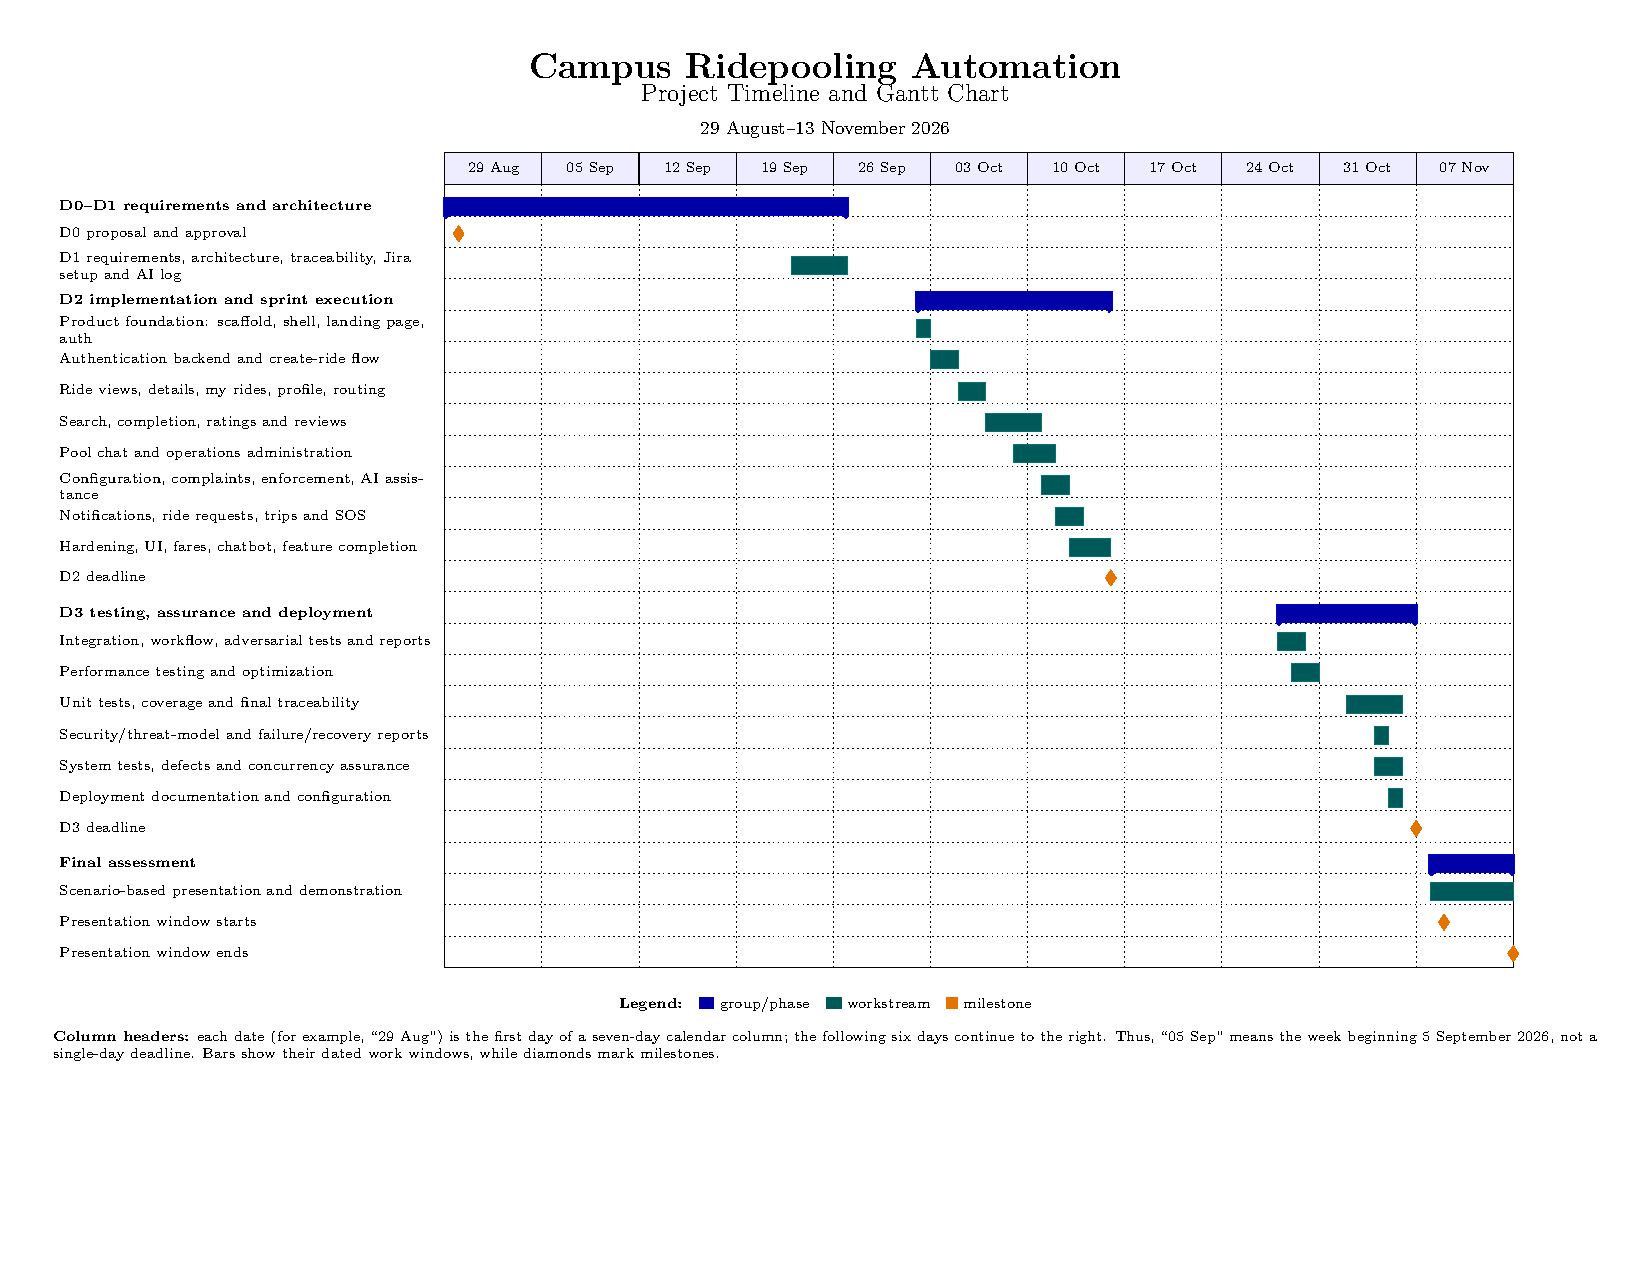
\includegraphics[width=\linewidth,height=0.92\textheight,keepaspectratio,trim=0 100 0 0,clip]{../project-timeline-gantt.pdf}
\caption{Project timeline and Gantt chart, from the
\repolink{Deliverables/D3/project-timeline-gantt.pdf}{timeline document}.}
\label{fig:gantt}
\end{figure}
\end{landscape}
